%%%%%%%%%%%%
%
% $Autor: Wings $
% $Datum: 2019-03-05 08:03:15Z $
% $Pfad: TemplateSensor $
% $Version: 4250 $
% !TeX spellcheck = en_GB/de_DE
% !TeX encoding = utf8
% !TeX root = filename 
% !TeX TXS-program:bibliography = txs:///biber
%
%%%%%%%%%%%%

\chapter{Schalter}

Um das Tischförderband mit Strom zu versorgen und den Modus der Förderrichtung zu wählen werden zwei verschiedene Kippschalter verwendet. 
\begin{itemize}
	\item Der in dem Tischförderband zur Stromversorgung verbaute Kippschalter, oder auch Wechselschalter, ist ein Schalter vom Typ \glqq SPDT \grqq. Dieser hat einen Anschluss, welcher an den Stromkreis angeschlossen ist und zwei Umschaltkontakte. Die beiden Umschaltkontakte werden an dieser Stelle verwendet, um den Stromkreis zu schließen, bzw. zu unterbrechen. 
	%\cite{}
	Dieser Kippschalter hat drei Pins und kann mit einer maximalen Schaltleistung von 30A/250V betrieben werden. Die folgende Abbildung \ref{pic:KippschalterEINEIN} zeigt diesen Kippschalter.
\end{itemize}

\begin{figure}
	\begin{center}
	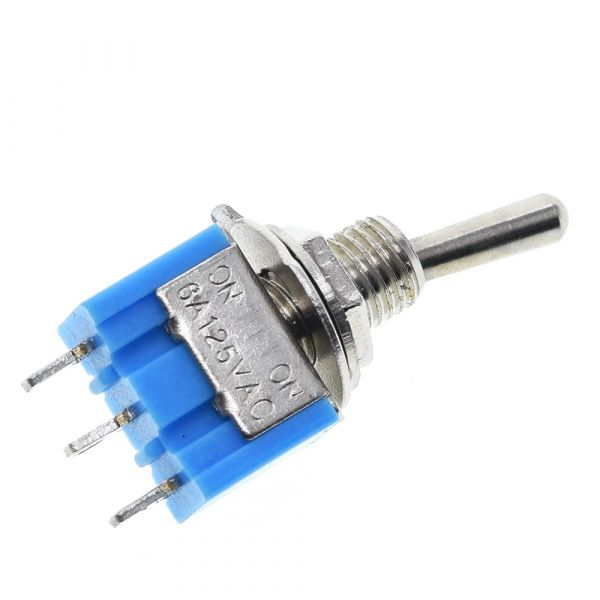
\includegraphics [width=50mm] {../../Images/BOM/KippschalterSPDTEinEin.jpg}
	\caption{Kippschalter \glqq EIN-EIN \grqq }
	\label{pig:KippschalterEINEIN}
	\end{center}
\end{figure}

\begin{itemize}
	\item Für die Moduswahl der Förderrichtung des Tischförderbands wird ein einpoliger Kippschalter mit drei Schaltzuständen (EIN-AUS-EIN) verbaut. Dieser ist ebenso wie der erste Kippschalter vom Typ \glqq SPDT \grqq, allerdings mit einer zusätzlichen Mittelstellung. Ist die Mittelstellung dieses Kippschalters betätigt, so ist kein Stromkreis geschlossen.  Die Belastungsgrenze des Schalters liegt bei 125 V bzw. 6 A. Die Feinsilberkontakte können verlötet werden oder per Steckverbindungen in den Stromkreis integriert werden. 
\end{itemize}

\begin{figure}
	\begin{center}
		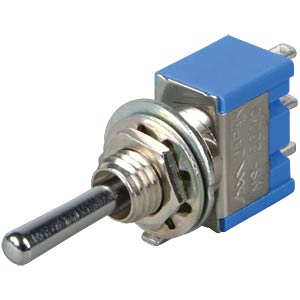
\includegraphics [width=50mm] {../../Images/BOM/KippschalterEinAusEin.jpg}
		\caption{Kippschalter \glqq EIN-AUS-EIN \grqq }
		\label{pig:KippschalterEINAUSEIN}
	\end{center}
\end{figure}